\documentclass{article}

\usepackage[utf8]{inputenc}
\usepackage[T1]{fontenc}
\usepackage[french]{babel}
\usepackage{graphicx}
\usepackage{caption}

% =====================
% DOCUMENT INFORMATION
% =====================
\title{Proc-8-bits - Conception d'un processeur avec jeu d'instructions élémentaires - v1.0}
\author{David DEVANT - Aurélien TROMPAT}
\date{\today}

\begin{document}
    % =====================
    % FRONT MATTER
    % =====================
    \maketitle

    \tableofcontents

    \section*{Introduction}
    \par L'objectif de ce projet est de concevoir un processeur 8 bits disposant d'un jeu de 4 instructions élémentaires : Non-OU, Addition, Stockage mémoire, Saut d'adresse  
    \newpage

    % =====================
    % MAIN MATTER
    % =====================
    \section{Architecture}
    \par L'architecture de notre CPU est imposée par le cahier des charges. Elle se divise en 3 parties :
    \begin{itemize}\renewcommand{\labelitemi}{$\bullet$} 
        \item Contrôleur (UC) : il est l'unité de contrôle qui génère des signaux internes de commandes. 
        \item Calculateur (UT) : Il effectue des calculs sur des données d'entrée et retourne de résultat vers la mémoire.
        \item Mémoire : Elle stocke le programme et les variables.
    \end{itemize}

    \section{Architecture CPU}
    \begin{figure}[h]
        \centering
        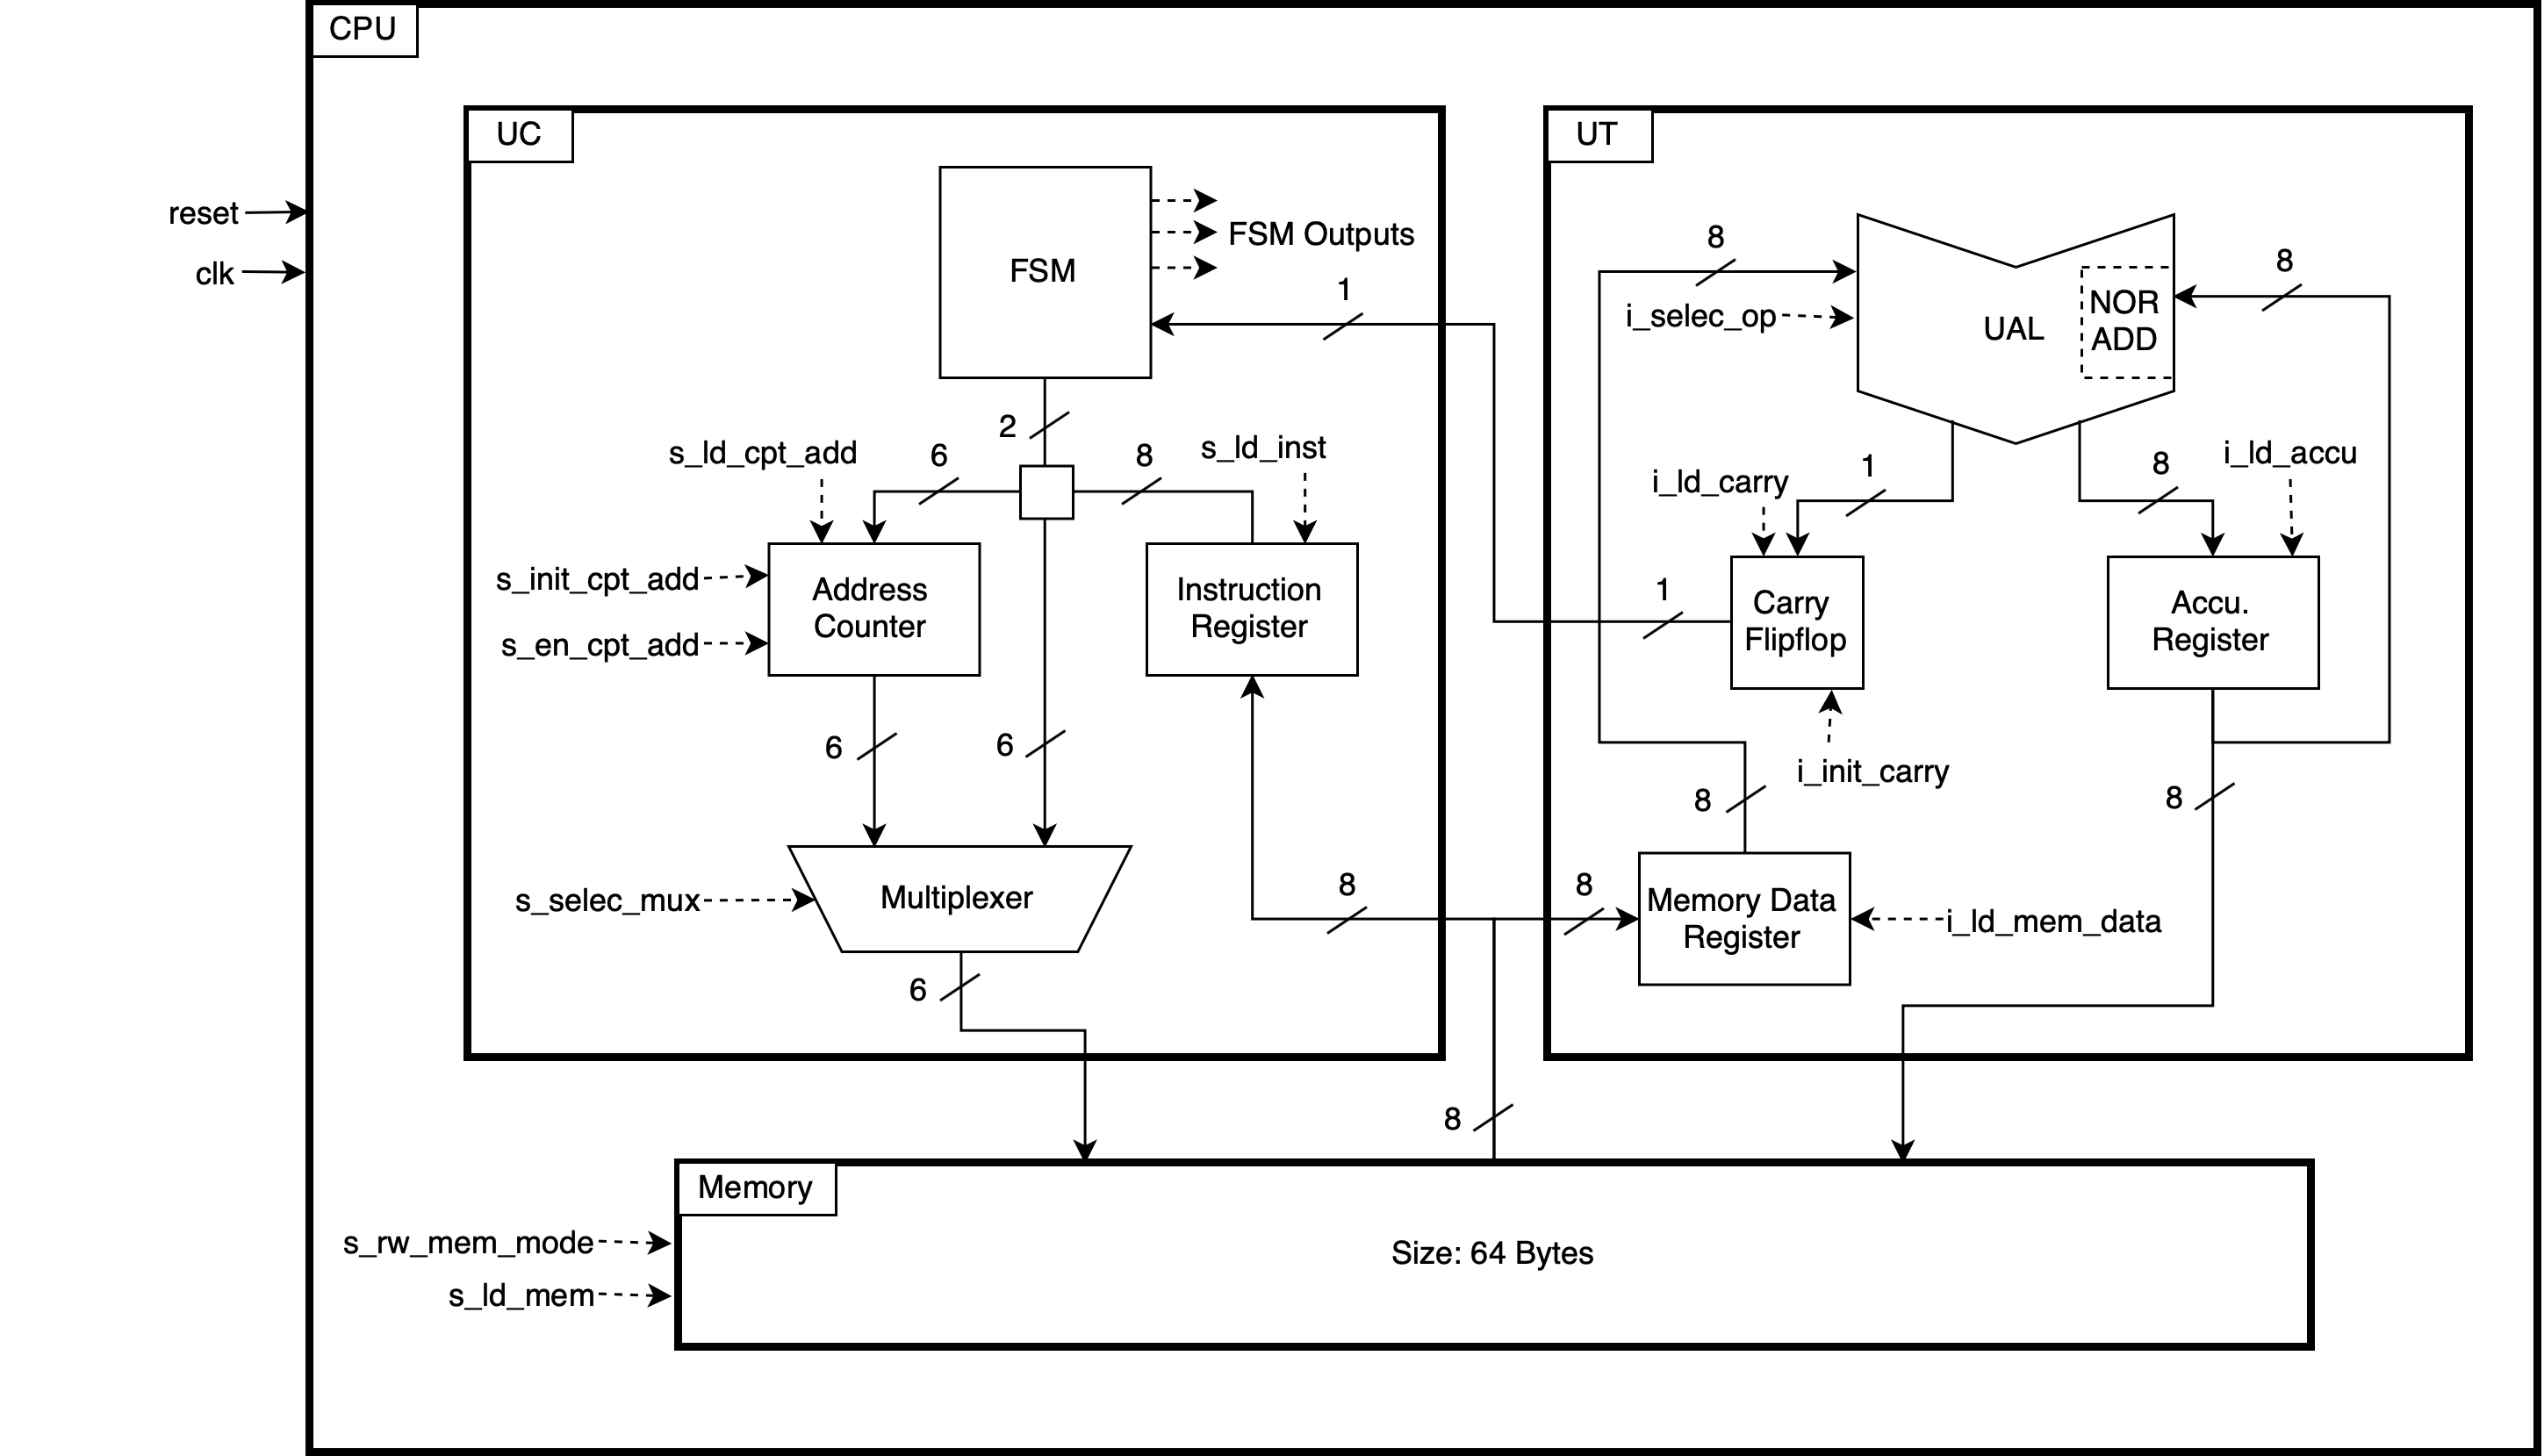
\includegraphics[width=\textwidth]{../doc/VHDL_Diagram.png}
        \caption{Architecture du CPU (Clock et reset non représenté)}
        \label{fig:vhdl_diagram}
    \end{figure}
    \subsection{Contrôleur (UC)}
    \subsubsection{Registre d'instruction}
    \par Il permet de stocker l'instruction qui est actuellement traitée par le CPU. Les instructions sur 8 bits sont issues de la mémoire. 
    \subsubsection{Compteur d'adresse}
    \par Ce compteur permet de définir l'adresse mémoire de la prochaine instruction que devra exécuter le CPU. Un système de chargement permet de modifier la valeur courante du compteur pour permettre des sauts d'adresse (Instruction JCC). Une entrée "init" permet de remettre à 0 le compteur pour redémarrer le programme à l'adresse 0.
    \subsubsection{Multiplexeur}
    \par Le multiplexeur est un composant purement combinatoire qui permet de sélectionner la source de l'adresse mémoire à lire/écrire. Si son signal de commande est à '0', alors c'est la sortie du compteur d'adresse qui est connecté à la mémoire. Ceci permet de lire les instructions du programme. Lorsque le signal de commande est positionné à '1', ce sont les 6 bits de poids faibles qui fixent l'adresse. Ceci permet d'effectuer les accès mémoire pour la partie calcul. 
    \subsubsection{Machine d'état (FSM)}
    \par La FSM est l'ordonnanceur du CPU. Elle génère 12 signaux qui commandent les différents composants du CPU. Voici son schéma: 
    \begin{figure}[h]
        \centering
        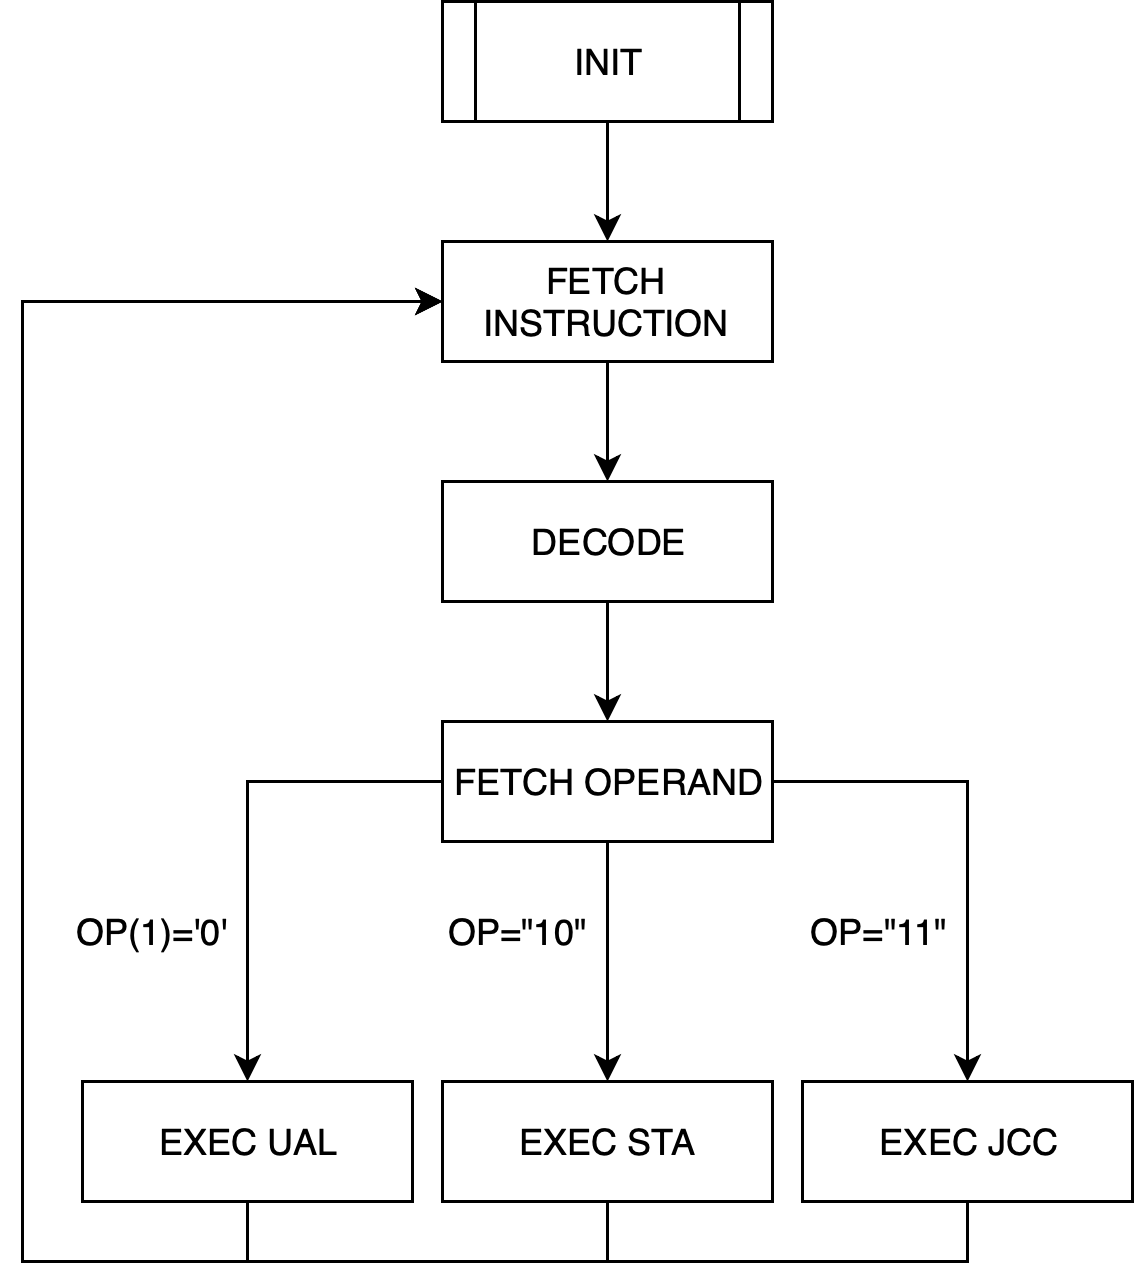
\includegraphics[width=200px]{../doc/FSMDiagram.png}
        \caption{Diagramme de la machine d'état du CPU}
        \label{fig:fsm_diagram}
    \end{figure}
    \begin{itemize}\renewcommand{\labelitemi}{$\bullet$} 
        \item INIT : Phase d'initialisation du CPU, cette étape n'est active qu'après un reset. 
        \item FETCH INSTRUCTION : Chargement de l'instruction indiquée par le compteur d'adresse.
        \item DECODE : Lit le code opération de l'instruction et anticipe un chargement de mémoire.
        \item FETCH OPERAND : Chargement de la variable pointée par l'instruction de la mémoire vers la partie opérative (UT). Le choix de l'étape suivante est conditionné par le code d'opération.
        \item EXEC UAL (Code OP = "00" ou "01") : Défini l'opération à effectuer sur la partie opérative puis ordonne la sauvegarde du résultat dans le registre d'accumulation. 
        \item EXEC STA (Code OP = "10") : Sauvegarde la valeur du registre d'accumulation en mémoire à l'adresse indiquée par l'instruction.
        \item EXEC JCC (Code OP = "11") : Effectue un test sur la valeur de la retenue pour déterminer si le saut d'adresse doit être exécuté. Le saut est effectué en plaçant les 6 bits de poids faible de l'instruction dans le compteur d'adresse.
    \end{itemize}
    \subsection{Contrôleur (UT)}
    \subsubsection{Registre de données mémoire}
    \par Ce registre permet de stocker la dernière valeur lue en sortie de la mémoire. Il est directement lié à l'unité de calcul UAL.
    \subsubsection{Registre d'accumulation}
    \par Ce registre stocke le résultat de la partie UAL. Sa valeur peut être envoyée vers la mémoire pour être sauvegardée ou bien réutilisée pour le calcul suivant.
    \subsubsection{Unité de calcul (UAL)}
    \par Cette unité de calcul dispose d'une entrée de sélection d'opération entre l'addition et le Non-OU. L'opération selectionnée est appliquée entre les deux valeurs 8 bits placées en entrée et le résultat est retourné vers le registre d'accumulation. Une seconde sortie permet de récupérer la retenue sur 1 bit pour être dirigée vers la flipflop.
    \subsubsection{Flipflop de retenue (Carry)}
    \par Cette bascule de type flipflop permet de stocker l'état de la retenue du dernier calcul de l'UAL. Sa sortie est utilisée par la FSM pour déterminer si le saut d'adresse de l'instruction JCC doit être effectué.
    \subsection{Mémoire}
	\par Cette mémoire de 64 octets est une mémoire simple accès avec un port de lecture et un second d'écriture. Elle est adressée sur 6 bits et manipule des valeurs sur 8 bits.
	
	\section{Tests}
    \par Chaque composant a été testé indépendemment à l'aide de "testbench". Une fois fonctionnels, nous les avons implémentés dans le top layer "CPU". Pour valider le projet, nous avons écrit les deux programmes de test vu en cours dans des fichiers "*.data". Ces fichiers sont chargés dans la mémoire juste avant la simulation. En observant les derniers accès mémoire du programme, on observe que les résultats sont cohérent avec les résultats attendus.
    \subsection{Additionneur N-bits}
    \begin{figure}[h]
        \centering
        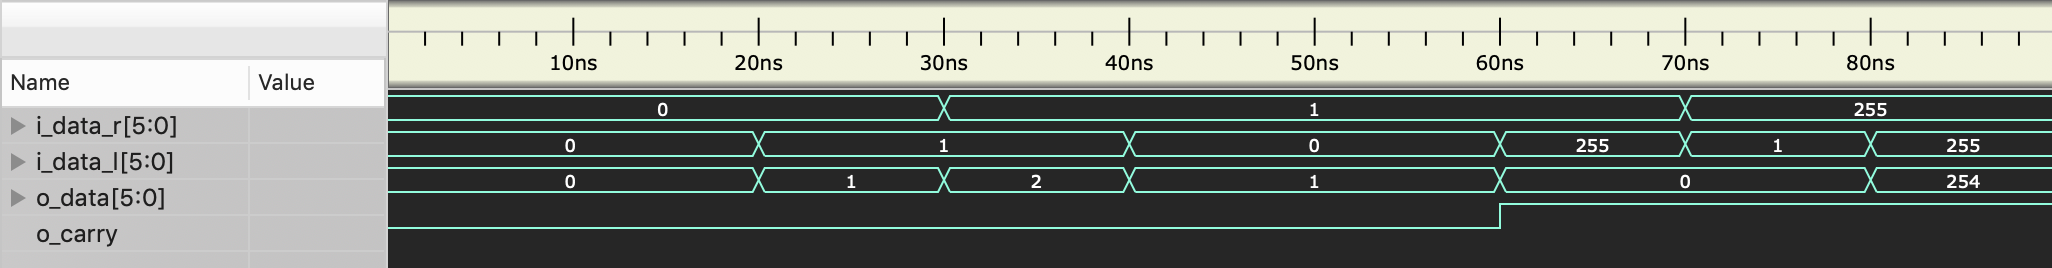
\includegraphics[width=\textwidth]{../doc/tb_screen/addi_n_bits.png}
        \caption{Diagramme temporel de l'additionneur N-bits}
        \label{fig:diag_tb_addi_n_bits}
    \end{figure}

    \subsection{Flipflop}
    \begin{figure}[h]
        \centering
        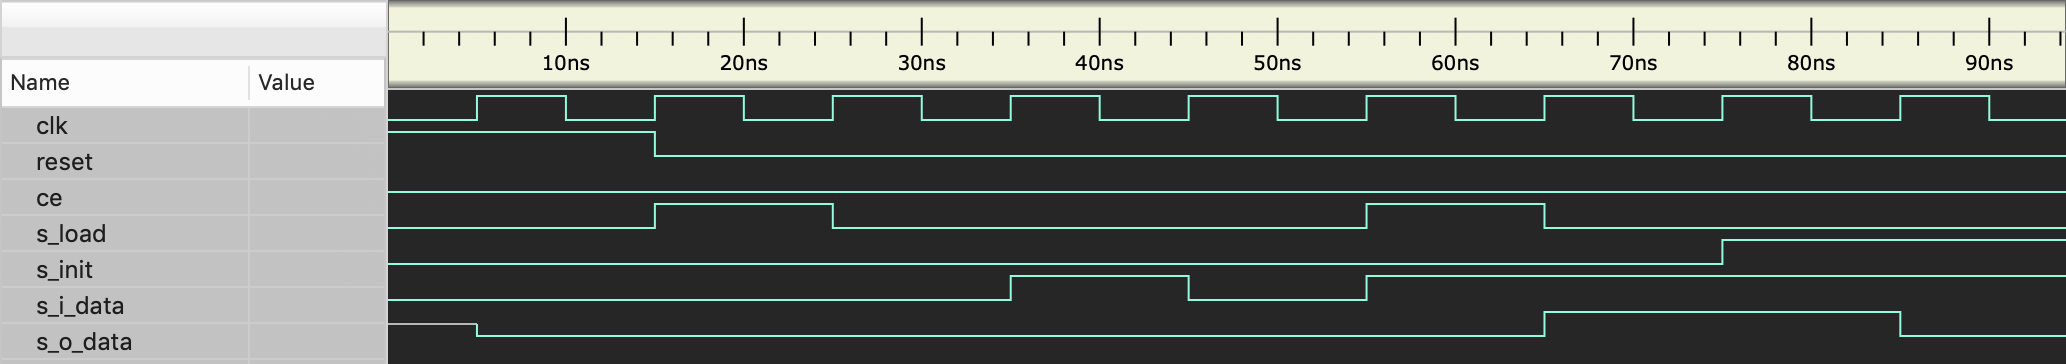
\includegraphics[width=\textwidth]{../doc/tb_screen/flipflop.png}
        \caption{Diagramme temporel de la flipflop de retenue}
        \label{fig:diag_tb_flipflop}
    \end{figure}

    \subsection{Multiplexeur à 2 entrées}
    \begin{figure}[h]
        \centering
        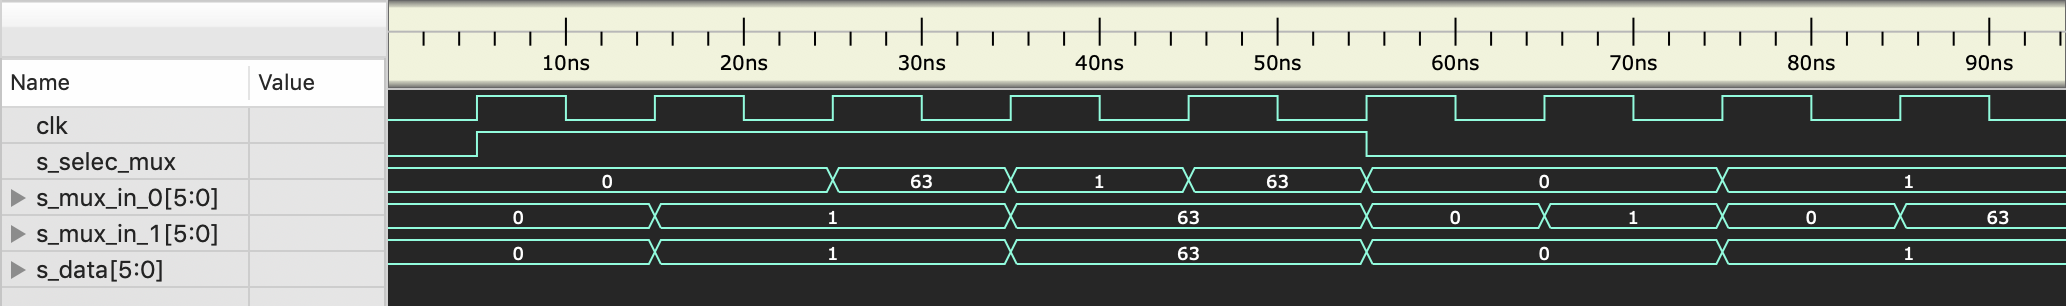
\includegraphics[width=\textwidth]{../doc/tb_screen/mux_2_in.png}
        \caption{Diagramme temporel du multiplexeur}
        \label{fig:diag_tb_mux_2_in}
    \end{figure}

    \subsection{Unité de calcul}
    \begin{figure}[h]
        \centering
        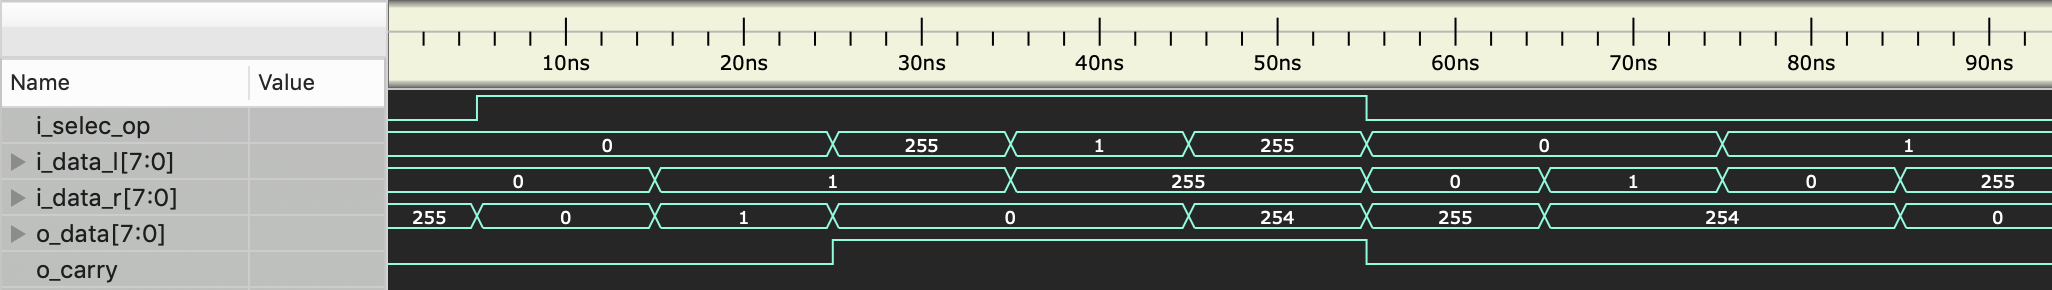
\includegraphics[width=\textwidth]{../doc/tb_screen/ual.png}
        \caption{Diagramme temporel de l'unité de calcul UAL}
        \label{fig:diag_tb_ual}
    \end{figure}

    \newpage
    
    \subsection{CPU - Programme du PGCD}
    \begin{figure}[h]
        \centering
        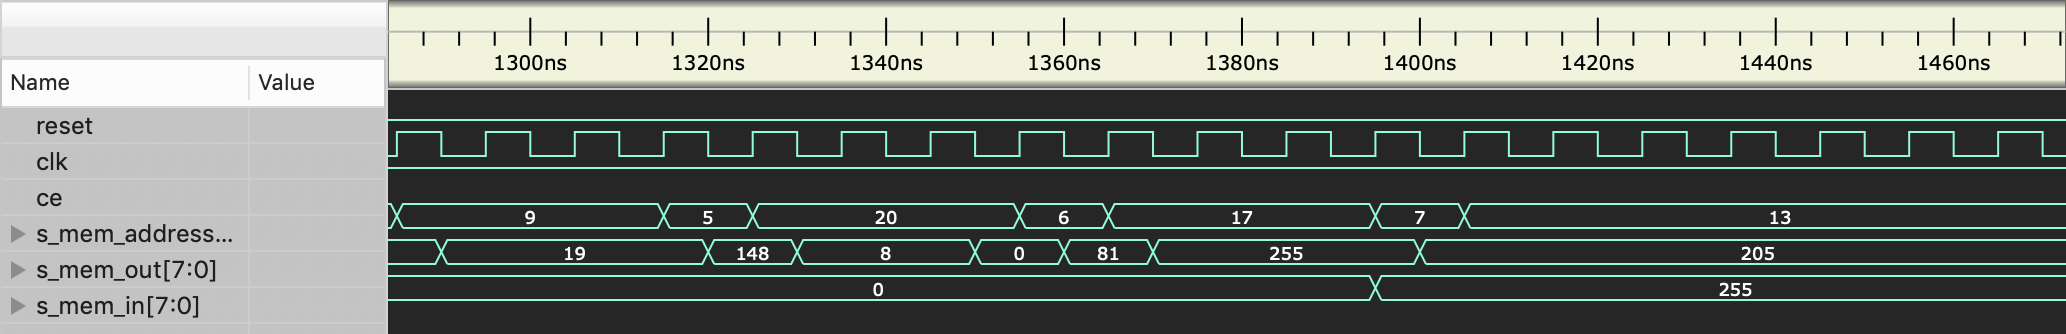
\includegraphics[width=\textwidth]{../doc/tb_screen/cpu_2nd_prog.png}
        \caption{Diagramme temporel du CPU avec programme de PGCD}
        \label{fig:diag_tb_cpu_2nd_prog}
    \end{figure}

    \subsection{FSM}
    \begin{figure}[h]
        \centering
        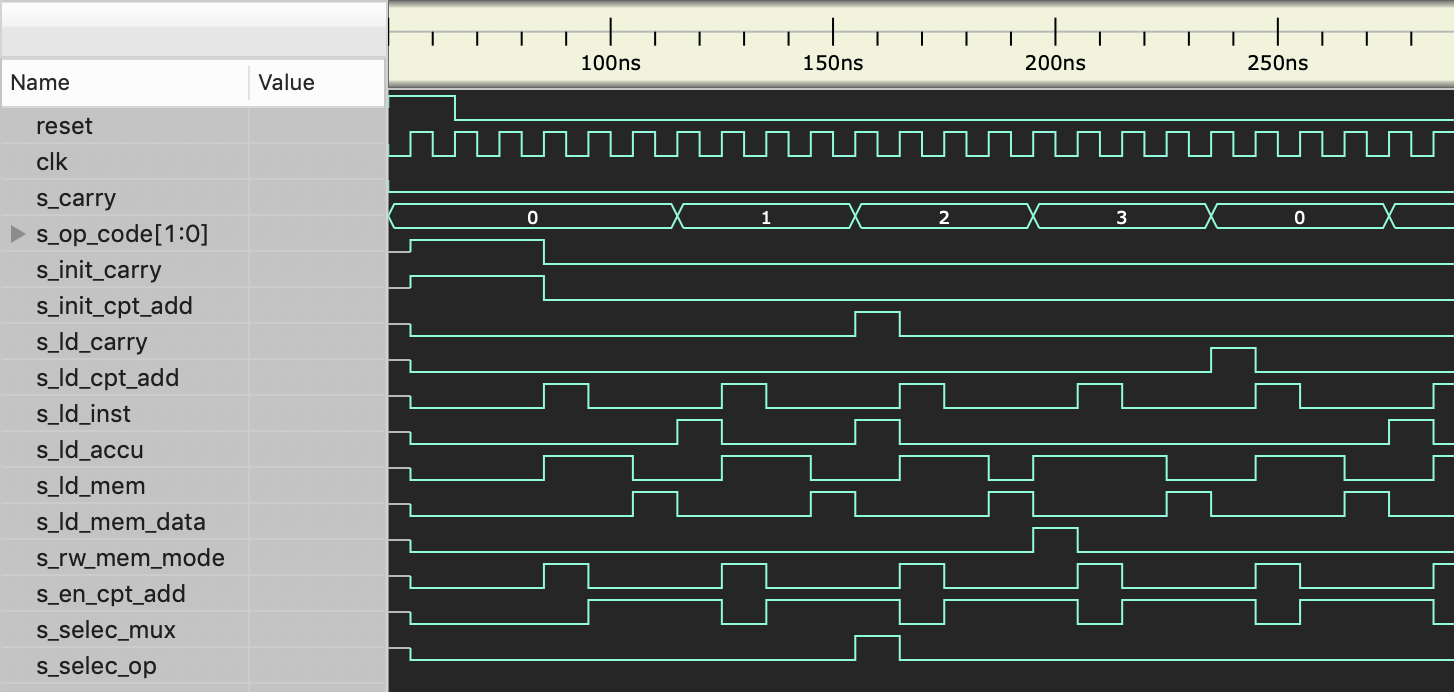
\includegraphics[width=\textwidth]{../doc/tb_screen/fsm.png}
        \caption{Diagramme temporel de la FSM}
        \label{fig:diag_tb_fsm}
    \end{figure}

    \newpage

    \section{Conclusion}
    \par Ce projet nous a fait découvrir les fonctionnements internes d'un processeur ainsi que les problématiques d'accès mémoire. L'implémentation en VHDL nous a permis de se remémorer les bonnes pratiques des langages de description. De plus, la réutilisation des nos anciens composants VHDL nous a montré qu'il était important de bien structurer et bien documenter nos fichiers pour être plus efficaces dans nos futurs projet.

    % =====================
    % BACK MATTER
    % =====================
\end{document}